Finalmente, con toda la información obtenida en los apartados anteriores, procedemos a desarrollar un protocolo de compensación de la variación de la ganancia debido a la temperatura. Nuestro objetivo es que, ante una modificación de la ganancia debida a una variación de la temperatura ambiente (por ejemplo debido a variaciones climatológicas) aplicar una variación adecuada en el voltaje operacional que devuelva a la ganancia a su valor inicial.

Como ya se ha explicado anteriormente, la importancia de este estudio de compensación radica en que deseamos utilizar el detector  a modo de alarma. Dado que este estará expuesto a condiciones climáticas arbitrarias, inevitablemente sufrirá variaciones de temperatura. Si queremos que el detector final sea capaz de avisar en caso de obtener una señal demasiado grande y que esta señal se corresponda a una fuga de tritio, necesitamos que el sistema posea una ganancia constante.

Las expresiones que se han obtenido con las dos calibraciones anteriores son:
\begin{equation}
G(V_{op})=cV_{op}+d; \qquad G(T)=aT+b
\label{gananciatotal}
\end{equation}

Esto implica que una variación de la ganancia en cada una de estas magnitudes viene dada como:
\begin{equation}
\partial G(V_{op}) = c \partial V_{op}; \qquad \partial G(T) = a \partial T
\label{variacionparcialganancia}
\end{equation}

Finalmente, la variación total de la ganancia ante una variación de ambas magnitudes viene dada por:
\begin{equation}
\partial G_{tot} = \partial G(V_{op}) + \partial G(T)
\label{variaciontotalganancia}
\end{equation}

Por tanto, si queremos que el valor de la ganancia se conserve ante una variación de ambas magnitudes, tenemos que conseguir que: 
\begin{equation}
\partial G_{tot} = 0 =  \partial G(V_{op}) + \partial G(T) \longrightarrow \partial G(V_{op}) = -\partial G(T)  
\label{basecompensacion}
\end{equation}
En otras palabras, debemos producir una  variación opuesta  de la ganancia con la modificación del voltaje a la que se ha producido al variar la temperatura. Para determinar esta variación, únicamente sustituimos las expresiones anteriormente obtenidas para cada diferencial de la ganancia:
\begin{equation}
\partial G(V_{op}) = - \partial G(T)  \longrightarrow c \partial V_{op}= - a \partial T \longrightarrow  \partial V_{op}= - \frac{a}{c} \partial T
\label{compensacionparciales}
\end{equation}
En trabajos anteriores\cite{TFMSiPM2, tesisSiPM, cladtesis} se ha visto que ambas pendientes, $a$ y $c$, apenas varían en voltaje y temperatura. Por tanto, en primera aproximación, podemos considerarlas constantes en ambas magnitudes. Con ello integramos a cada lado y obtenemos:
\begin{equation}
\int_{V_i}^{V_f} \partial V_{op}= - \frac{a}{c} \int_{T_i}^{T_f}\partial T = - \frac{a}{c} \Delta T \longrightarrow \Delta V_{op}= e \Delta T
\label{integral}
\end{equation}
donde se ha introducido un nuevo parámetro: $$e=-\frac{a}{c}$$ cuyo valor se obtiene de las ecuaciones $\eqref{ajustependientetemperatura}$  y $\eqref{ajustependientevoltaje}$:
\begin{equation}
c=(234.1 \pm 2.6) \cdot 10^6~\volt^{-1}
\label{pendientevoltaje}
\end{equation}
\begin{equation}
a=(-140.3 \pm 2.7) \cdot 10^5~\frac{1}{\celsius}
\label{pendientetemperatura}
\end{equation}
\begin{equation}
e=-\frac{a}{c} = (59.9 \pm 1.3) \cdot 10^{-3} \quad \volt  \celsius^{-1}
\label{pendientecompensacion}
\end{equation}
donde el error de $e$ se ha obtenido mediante propagación de errores. 

Finalmente, procedemos a analizar el resultado. Hemos obtenido dos dependencias de la ganancia lineales y opuestas. Por un lado la ganancia disminuye con la temperatura y por otro lado la ganancia aumenta con el voltaje operacional. Por tanto, si queremos conseguir modificaciones opuestas de la ganancia debemos desplazar voltaje y temperatura en la misma dirección (aumentar o disminuir ambas magnitudes simultáneamente). Si analizamos el resultado vemos que, efectivamente, tenemos una dependencia positiva.
También apreciamos que obtenemos un valor dos órdenes de magnitud inferior a la unidad. Esto es debido a que la dependencia de la ganancia con el voltaje es mucho más marcada que la variación con la temperatura (mayor pendiente en valor absoluto para el ajuste del voltaje que para el ajuste de la temperatura). Este es el motivo por el que se toma pasos más reducidos para el voltaje que para la temperatura. 

En resumen, la ecuación que nos dicta cual es la variación que debemos aplicar al voltaje para mantener un valor de ganancia constante (compensar la ganancia) ante una variación de la temperatura conocida (que puede ser medida con un sensor de temperatura) es:
\begin{equation}
\Delta V_{op}=0.059929 \cdot \Delta T \longrightarrow V_1-V_{ref}=0.059929(T_1-T_{ref})
\label{compensacionfinal}
\end{equation}
Donde $V_1$ es el voltaje con el que hay que alimentar al SiPM a una temperatura ambiental de $T_1$ para mantener la ganancia constante a su valor de referencia. Para realizar este cálculo, se necesita tomar un valor de voltaje operacional y temperatura como referencía, cuya ganancia es la que mantendremos. Para estos valores de referencia elegiremos el caso anteriormente mostrado en la sección de análisis de datos correspondiente a temperatura $25~\celsius$, humedad del $45\% $ y voltaje operacional de $53.97~\volt = V_{BD}+ 3~\volt$ , cuya ganancia total hemos visto que corresponde a $7.18235 \cdot 10^8$. Por tanto, el valor de voltaje operacional $V_1$ con el que hay que alimentar un SiPM a temperatura $T_1$, para mantener una ganancia de $7.18235 \cdot 10^8$ es:
\begin{equation}
V_1=0.059929T_1+52.47
\label{compensacionfinal}
\end{equation}




Procedemos a realizar una verificación midiendo los casos de $21, 23, 25, 27$ y  $29~\celsius$. En cada uno de ellos se corregirá el voltaje de alimentación de forma adecuada para mantener el mismo valor de la ganancia. El valor de la ganancia medida para cada caso se muestra en la figura~\ref{compensacion}. 

\begin{figure}[hbtp]
\centering
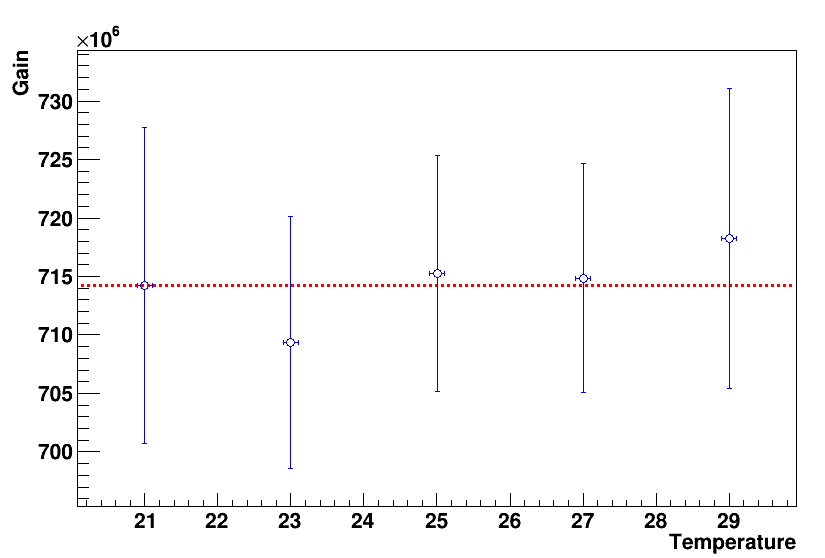
\includegraphics[scale=0.4]{compensacion.png}
\caption{Ganancia frente a temperatura después de corregir con el voltaje de operacion.\label{compensacion}}
\end{figure}
donde la raya roja corresponde al ajuste a una constante. Su valor, correspondiente al valor de la ganancia es $G=(714.2 \pm 4.9) \cdot 10^6$. Comprobamos la calidad del ajuste a partir del test $\chi^2$ obteniendo un valor de $\frac{\chi^2}{ndf}=\frac{0.318}{4}\approx 0.0795$, valor ligeramente bajo, probablemente debido a una sobreestimación de los errores (algo que ya puede apreciarse en la imagen).

Vemos que el método funciona de manera muy eficaz, ya que la ganancia presenta variaciones muy pequeñas de aproximadamente $\Delta G=5 \cdot 10^6$, que corresponde a una variación relativa de $\sigma_{rel}=0.28\%$. Hemos comprobado por tanto que se trata de un método realmente eficaz.

La máxima variación se observó a $23~\celsius$, debido a que fue una medida realizada muchas horas después de tomarse las otras y existen factores externos que no podemos controlar que afectan al sistema. En este tiempo más largo transcurrido es más probable que hayan cambiado estos factores. Sin embargo, puede observarse en todo momento que la variación de la ganancia es mínima verificando en gran medida la ecuación anteriormente obtenida.

